\chapter{RESEARCH METHODOLOGY}
\label{ch:method}

This chapter details the strategy adopted in this study to achieve the study objectives. The aim of the research method section is to explain the techniques and processes employed in the investigation, along with their operational mechanisms.
\section{Research Framework}
The Research Methodology is the orderly process and strategy employed in conducting research, gathering information, inspecting material, and drawing conclusions. It encompasses a range of methodologies, processes, tools, and tactics that researchers use to meet their research objectives or questions. 

The methodology section of the research provides a rundown of the steps and procedures followed in the study, encompassing the research design, sampling strategies, data analysis methods, and ethical concerns. It offers a systematic framework for conducting and presenting research across diverse academic disciplines, assisting in the maintenance of rigor, validity, and reliability in the research results. The research framework for this study is designed to follow a systematic and iterative process.

The study has been conducted in multiple stages, progressing from initial preliminary studies, to acquisition of data, pre-processing of data, the development of the machine learning model, proceeded by the evaluation of the model and finally the documentation. The figure below presents a visualization of the research.


\begin{figure}[h]
    \centering
    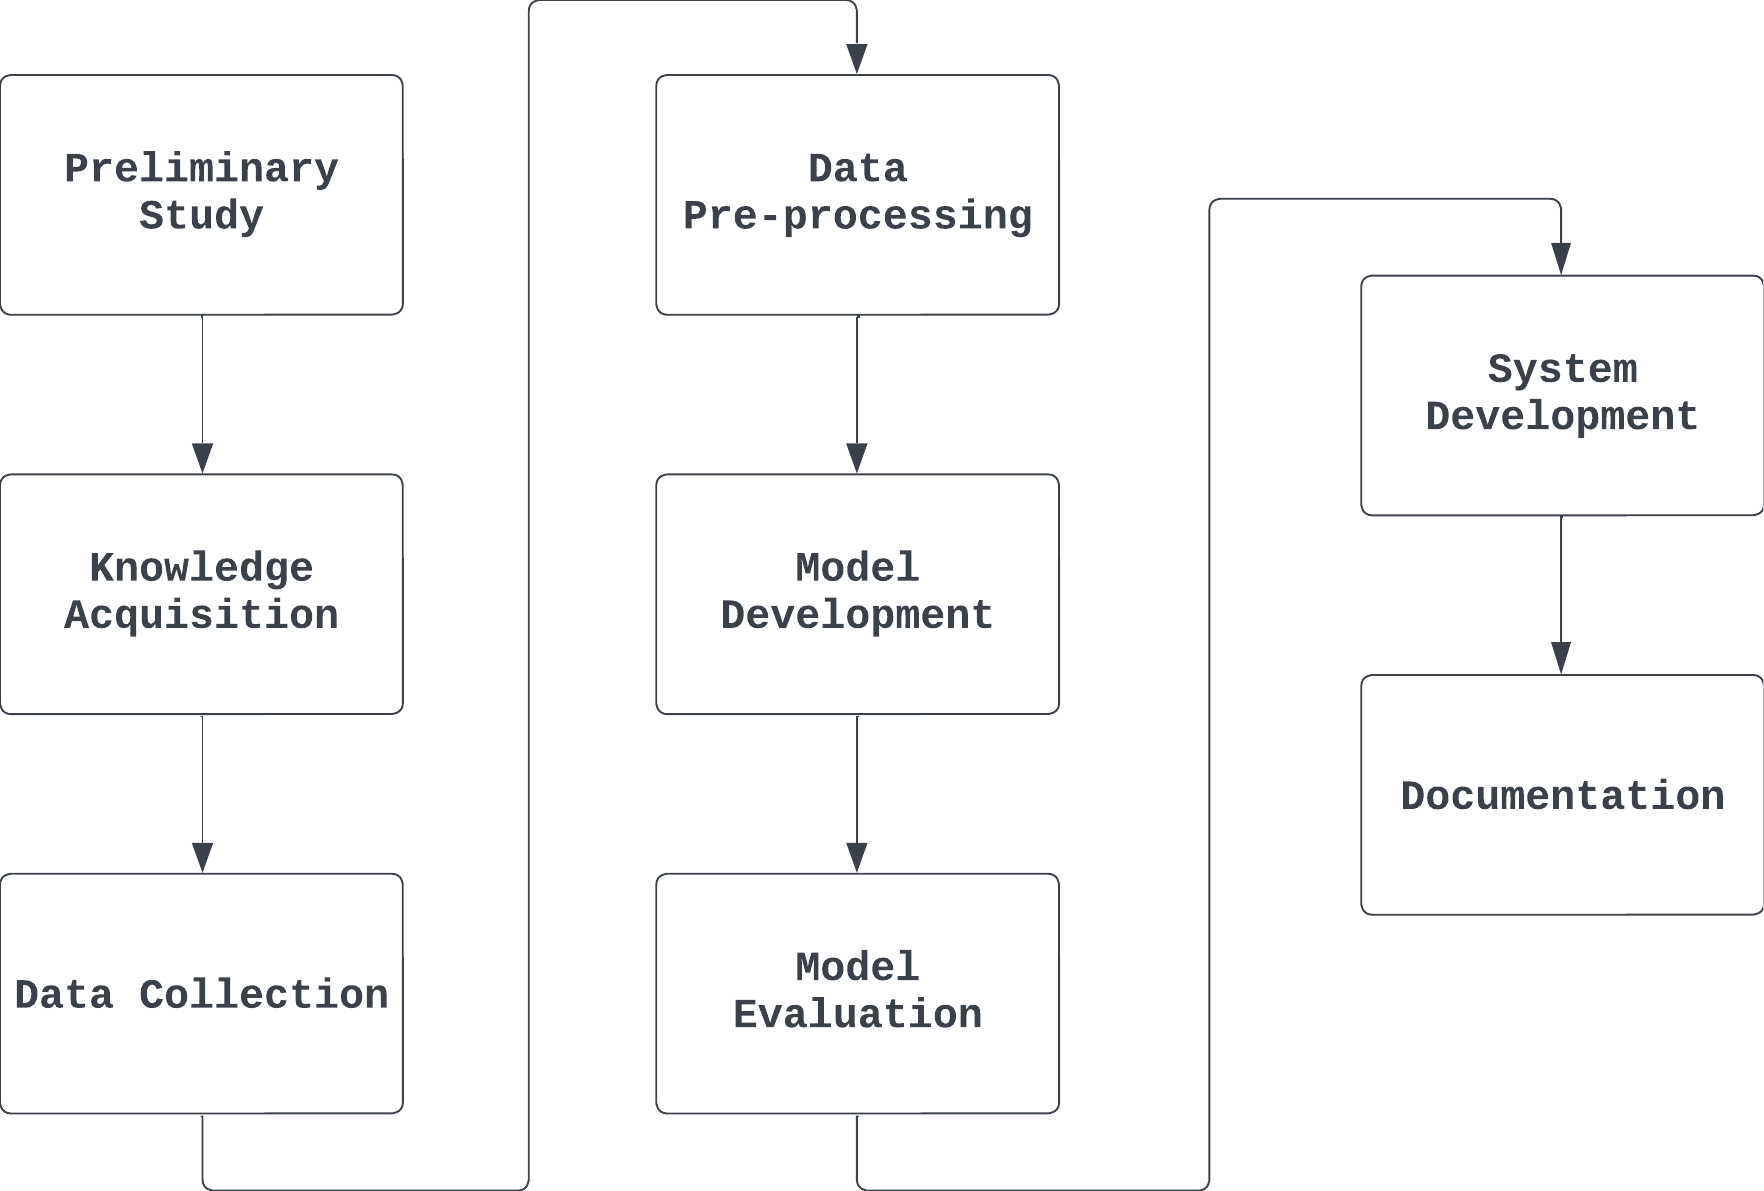
\includegraphics[scale=0.75]{mainmatter/images/research methodology/MPN.png}
    \caption{Methodology Phases}
    \label{fig:methodologyphases}
\end{figure}
\newpage
The following table presents a compilation of various research inquiries that have been raised to address the problem statement outlined in Chapter 1.


\begin{longtable}{|p{5cm}|p{7.5cm}|}
\caption{Research Questions.} \label{table:researchquestions}\\
\hline
\textbf{Questions} & \textbf{Description} \\ [0.5ex] 
\hline
\endfirsthead
\hline
\endhead
\hline
\endfoot
\endlastfoot
How do we differentiate between dyslexic and non-dyslexic handwriting? & To identify the features of dyslexia handwriting in images. \\
\hline
How to create machine learning model that can identify dyslexic and non-dyslexic handwriting? & To develop a machine learning model to distinguish dyslexic or non-dyslexic samples. \\
\hline
How do we view the performances of the machine learning model? & To evaluate the performance of the machine learning model. \\
\hline
\end{longtable}
 The problem statement discussed in Chapter 1 has resulted in several research questions. One of these questions explores the performance evaluation of a machine learning model developed to differentiate between dyslexic and non-dyslexic handwriting samples, using metrics such as accuracy, precision, recall, and F1-score. Another research question pertains to conducting a literature review on the detection of dyslexic handwriting, aimed at gaining a comprehensive understanding of dyslexia's impact on handwriting and identifying gaps in existing methodologies. 

\newpage
In Table \ref{table:methodologyframework}, the table presents the methodology framework which includes the phases, activities, and deliverables for this report based on the study objectives.

\begin{longtable}{|p{3cm}|p{3cm}|p{3.5cm}|p{4cm}|}
    \caption{Methodology Framework.\label{long}}
\label{table:methodologyframework}\\
\hline
\textbf{OBJECTIVES} & \textbf{PHASES} & \textbf{ACTIVITIES} & \textbf{DELIVERABLES} \\ [0.5ex] 
\hline
\endfirsthead
\hline
\endhead
\hline
\endfoot
\endlastfoot

 \multirow{3}{3cm}{To identify the features of dyslexia handwriting in images.} & Preliminary Study & Examine and comprehend the study thoroughly. Pinpoint the research goal, determine its scope, and highlight the importance of the study. & Chapter 1: Background of Study, Problem Statement, Research Objectives, Scope of Study, Significance of Research\\\cline{2-4} 
 & Knowledge Acquisition & Review existing research on dyslexia, and its effect on handwriting. Discover relevant machine learning algorithms, and its tools. & Chapter 2: Literature Review \\\cline{2-4} 
 & Data Collection & Obtain data for the research from available resources. & Datasets to be used for dyslexic handwriting recognition. \\
 \hline
\multirow{2}{3cm}{To develop machine learning models to distinguish dyslexic or non-
dyslexic samples.} & Data Pre-processing & Process the raw datasets, and go through pre-processing procedures.  & Cleaned data. \\\cline{2-4} 
 & Model Development & Apply the LeNet-5 model & LeNet-5 model to be evaluated. \\
 
 \newpage
 \multicolumn{4}{c}%
{{\bfseries \tablename\ \thetable{} -- continued from previous page}} \\
\hline \multicolumn{1}{|c|}{\textbf{OBJECTIVES}} & \multicolumn{1}{c|}{\textbf{PHASES}} & \multicolumn{1}{c|}{\textbf{ACTIVITIES}} & \multicolumn{1}{c|}{\textbf{DELIVERABLES}} \\ \hline
 \multirow{3}{3cm}{To evaluate the performance of the machine learning model.} & Model Testing and Evaluation & Evaluate the performance of LeNet-5 & Performance of the LeNet-5 model. Result comparison and analysis. \\\cline{2-4} 
 & System Development & Develop the system and present a usable interface. & System that can be used. \\\cline{2-4}
 & Documentation & Document every step and process of the research. & Completed document to use as a reference. \\
 \hline

\end{longtable}


\newpage
\section{Preliminary Study}
Preliminary Study represents the initial phase where it involves a comprehensive exploration and understanding of the study's foundational elements, and in the context of this study, it primarily involved dyslexia and machine learning. This phase involved conducting domain and title searches for interested parties. To come up with a suitable and good title, it also entails having frequent interactions with supervisor(s). This is a safety measure done to prevent titles irrelevant to the subject matter being picked up. It is followed up by an in-depth research, carried out by reading credible articles and research papers with the aim of grasping and identifying the problem in the chosen domain.

\subsection{Problem Identification}
The problem identified in this study is that dyslexic handwriting detection currently relies on manual evaluation, which can be time-consuming and subjective. This approach results in potential delays in identifying dyslexic individuals and providing them with appropriate support. Therefore, there was a demand to implement machine learning techniques to accurately detect dyslexic handwriting.

\newpage
\subsection{Domains and Technique Understanding}

\subsubsection{Dyslexia}
Dyslexia is a neuro-developmental condition that presents challenges in acquiring reading skills, even with standard teaching methods, sufficient intelligence, and a well-rounded socio-cultural environment. According to \textcite{Wajuihian2011DyslexiaAO}, it is the most prevalent form of learning disorder, and its impact on reading abilities can significantly hinder a child's academic performance.

\subsubsection{Machine Learning}
Machine learning is a field that encompasses automated computational processes where logical or binary operations are utilized to enable computers to acquire knowledge and skills by studying numerous instances or examples. By employing sophisticated algorithms, machine learning systems can analyze and comprehend patterns, relationships, and data in order to enhance their performance and make informed predictions or decisions. This transformative technology, according to \textcite{Fulkerson1995}, has revolutionized various industries, especially in healthcare, by enabling computers to learn from experience and adapt their behavior accordingly.

\newpage
\section{Knowledge Acquisition}
To gather a thorough understanding of the study, firstly knowledge must be acquired. Knowledge acquisition is the stage where information is gathered primarily through review methods. It refers to the process of deriving knowledge and information from a multitude of sources to enhance understanding or facilitate decision-making. This acquisition of knowledge was accomplished through various means such as articles, interviews, surveys, literature reviews, and experimental research.

To enhance the process of knowledge acquisition, a systematic approach had been developed, which involved reviewing previous research and studies. This approach ensured a structured method of acquiring knowledge by categorizing research topics according to the following table. Each domain and technique within these categories has its own set of concepts that need to be read and analyzed in order to grasp the fundamental principles of each specific area. 

Once the fundamental concepts of each domain or technique were understood, the correlation and analysis of combining two domains or techniques come into play. This approach allowed for a deeper exploration of the subject matter by examining the connections and interactions between different domains or techniques.

For this project, a thorough study of dyslexia and machine learning was conducted. This involves performing a literature review on dyslexia, and its effect on handwriting, as well as discovering relevant machine learning algorithms, and its tools. The knowledge is acquired from online platforms, most notably Google Scholar, Semantic Scholar, and IEEE Xplore. As for IEEE Xplore, it is made accessible through UiTM's library website.

Related articles and research papers are then saved in Mendeley's reference manager, which is then used to organize the references, and to cite them in the documentation. In this context, the .bib file is exported from Mendeley, and is used in LaTeX to cite the references.



\newpage
\section{Data Collection}
Data collection is a systematic process of gathering relevant information and data points from various sources or individuals to aid in research, analysis, or in decision-making. This process involves identifying the necessary data, designing data collection methods such as surveys, interviews, observations, or experiments, and obtaining the data through structured or unstructured techniques. 

The nature of the data gathered can be either qualitative or quantitative, depending on the research objectives, and can originate from primary sources like direct participant interviews, or secondary sources such as pre-existing datasets, literature, or publicly available data.

In this study, a Kaggle dataset was being used for data collection, where there are a wide collection of datasets relevant to a sorts of studies being done. For this research, a dataset released from \textcite{Isa_2022_Kaggle} has been used. The dataset was gathered from 3 sources, which were from \textcite{datasetsrc1} for uppercase letters, while using \textcite{datasetsrc2} for lowercase letters and several testing datasets were obtained dyslexic kids of Seberang Jaya primary school, Penang, Malaysia. 

\begin{figure}[h]
    \centering
    
\includegraphics[scale=0.2]{mainmatter/images/research methodology/Kaggle_logo.png}
    \caption{Kaggle logo}
    \label{fig:kaggle-logo}
\end{figure}


\newpage
\section{Data Pre-processing}
The phase in focus is data pre-processing, a critical step used to transform raw data into an effective and efficient format for further use. Raw data from the dataset need to be processed prior to their application in training and testing procedures. 

Initially, the dataset used was designed to classify three types of handwriting, which are normal, reversal, and corrected handwriting. The tree structure of the dataset can be seen in Figure \ref{fig:oldtree}. This dataset contains a total of 78,275 images for normal class while for reversal are 52,196 images and for corrected are 8,029 images, which totals up to 138,500 images.

\begin{figure}[h]
    \centering
    \begin{forest}
        for tree={
            font=\ttfamily,
            grow'=0,
            child anchor=west,
            parent anchor=south,
            anchor=west,
            calign=first,
            edge path={
            \noexpand\path [draw, \forestoption{edge}]
            (!u.south west) +(7.5pt,0) |- node[fill,inner sep=1.25pt] {} (.child anchor)\forestoption{edge label};
            },
            before typesetting nodes={
            if n=1
                {insert before={[,phantom]}}
                {}
            },
            fit=band,
            before computing xy={l=15pt},
        }
        [Dataset
        [Train
            [Normal]
            [Corrected]
            [Reversal]
        ]
        [Test
            [Normal]
            [Corrected]
            [Reversal]
        ]
        ]
    \end{forest}
    \caption{Tree structure of the dataset}
    \label{fig:oldtree}
\end{figure}

\newpage
The dataset was then modified to only classify normal and potentially dyslexic handwriting, which consists of the combination of the correction and reversal class. The tree structure of the modified dataset can be seen in Figure \ref{fig:newtree}. With that, the dataset contains a total of 78,275 images for normal class and a total of 60,225 images for potentially dyslexic class.

\begin{figure}[h]
    \centering
    \begin{forest}
        for tree={
            font=\ttfamily,
            grow'=0,
            child anchor=west,
            parent anchor=south,
            anchor=west,
            calign=first,
            edge path={
            \noexpand\path [draw, \forestoption{edge}]
            (!u.south west) +(7.5pt,0) |- node[fill,inner sep=1.25pt] {} (.child anchor)\forestoption{edge label};
            },
            before typesetting nodes={
            if n=1
                {insert before={[,phantom]}}
                {}
            },
            fit=band,
            before computing xy={l=15pt},
        }
        [Dataset
        [Train
            [Normal]
            [Potential Dyslexia]
        ]
        [Test
            [Normal]
            [Potential Dyslexia]
        ]
        ]
    \end{forest}
    \caption{Tree structure of the modified dataset}
    \label{fig:newtree}
\end{figure}

As the dataset has been already pre-processed, the only pre-processing step taken was to apply the \texttt{rescale} function, in order to normalize the pixel values in the images to the range [0,1]. It is believed that it helps the model converge faster and prevents the gradients from becoming too large. Furthermore, as the training and testing dataset are already separated, no splitting of the dataset was required, with the exception of the validation dataset, which was 10\% of the testing dataset. The dataset was then loaded into the model, and the model was trained using the dataset.

\newpage
\section{Model Development}

For model development, Python was chosen as the preferred programming language. The reasoning behind this is as to utilise TensorFlow as the main framework. TensorFlow is an open-source software library for machine learning, which was developed by the Google Brain team. It is a symbolic math library, and is also used for machine learning applications such as neural networks. 

\begin{figure}[h]
    \centering
    
\includegraphics[scale=0.3]{mainmatter/images/research methodology/tf_logo.png}
    \caption{TensorFlow logo}
    \label{fig:tensorflow}
\end{figure}

This is assisted by using Keras, a high-level API that is built on top of TensorFlow. Keras is a deep learning API written in Python, which runs on top of TensorFlow, CNTK, or Theano. It was developed with a focus on enabling fast experimentation, and is designed to be user-friendly, modular, and extensible.

To smoothen the process of developing the model, the development is done locally on a Windows Subsystem for Linux 2 (WSL2) environment, running Ubuntu 22.04, codenamed `Jammy Jellyfish'. With that, it opens up for the use of GPU acceleration in TensorFlow, which is provided by NVIDIA CUDA. The specifications of the hardware used can be seen in Table \ref{table:hardware}.

\begin{longtable}{|p{3cm}|p{7.5cm}|}
\caption{Hardware Specifications.}
\label{table:hardware}\\
\hline
\textbf{Hardware} & \textbf{Description} \\ [0.5ex]
\hline
\endfirsthead
\hline
\endhead
\hline
\endfoot
\endlastfoot
CPU & AMD Ryzen 7 3700X 8-Core Processor \\ \hline
GPU & NVIDIA GeForce RTX 3060 12GB \\ \hline
RAM & 16GB 3200MHz DDR4 \\ \hline
\end{longtable}


In this study, a modified version of LeNet-5 has been used, a convolutional neural network (CNN) architecture that was developed by \textcite{Lecun1998}. The LeNet-5 architecture consists of 7 layers, which are 2 convolutional layers, 2 subsampling layers, 2 fully connected layers, and 1 output layer. 

However, for this study, the architecture has been modified to include BatchNormalization, where it improves accuracy, followed by applying MaxPooling2D, to produce smaller feature sizes. Besides that, a dropout layer is included to prevent overfitting. The architecture of the modified LeNet-5 can be seen in Figure \ref{fig:lenet5}.

\begin{figure}[h]
    \centering
    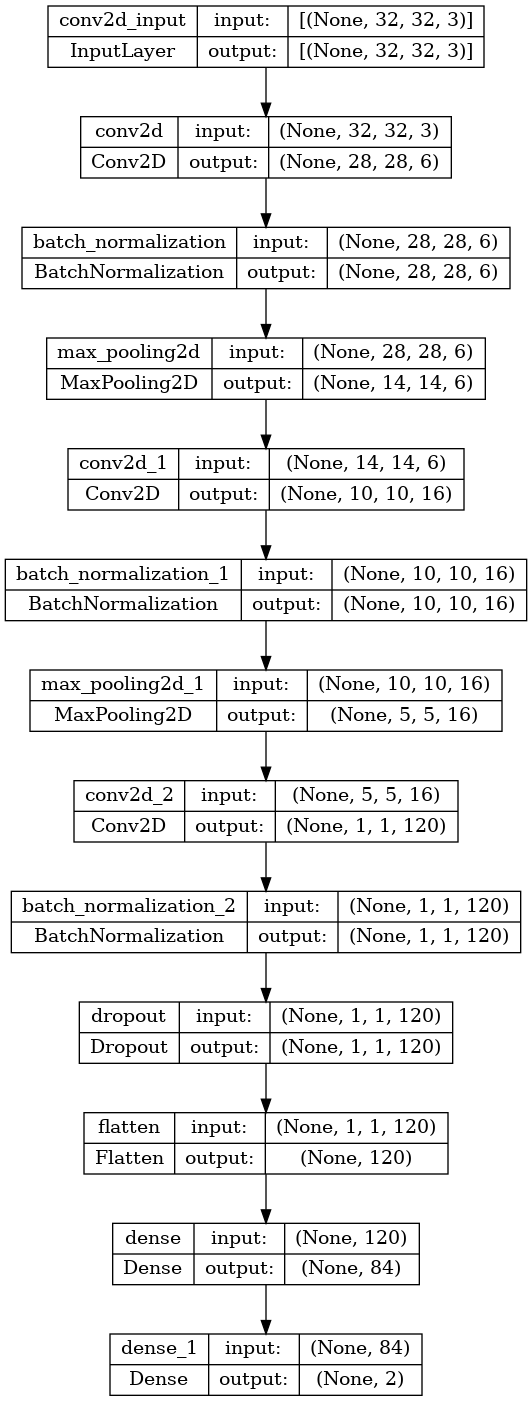
\includegraphics[scale=0.4]{mainmatter/images/research methodology/model.png}
    \caption{Modified LeNet-5 architecture}
    \label{fig:lenet5}
\end{figure}

\newpage
The model takes an input size of 32x32, which is the size of the images in the dataset. The breakdown of the layers can be seen in Table \ref{table:lenet5}.

\begin{longtable}{|p{3.75cm}|p{8cm}|}
\caption{Detailed description of the LeNet-5 model.}
\label{table:lenet5}\\
\hline
\textbf{Layer} & \textbf{Description} \\ [0.5ex]
\hline
\endfirsthead
\hline
\endhead
\hline
\endfoot
\endlastfoot
Input & Input layer, takes an input size of 32x32.\\ \hline
Conv2D & This initial convolutional layer applies 6 filters of size 3x3, extracting basic features from the input images. It has 456 trainable parameters. \\ \hline
BatchNormalization & This layer normalizes the activations of the first convolutional layer, stabilizing training and potentially accelerating convergence. \\ \hline
MaxPooling2D & This layer downsamples the spatial dimensions of the feature maps by a factor of 2, reducing computation and promoting invariance to small translations.\\ \hline
Conv2D & The second convolutional layer applies 16 filters of size 3x3, capturing more complex features. It has 2,416 trainable parameters.\\ \hline
BatchNormalization & This layer normalizes the activations of the second convolutional layer, similarly aiding training. \\ \hline
MaxPooling2D & This layer further downsamples the feature maps, enhancing spatial invariance and reducing overfitting. \\ \hline
Conv2D & The third convolutional layer applies 120 filters, further refining feature extraction. It has 48,120 trainable parameters.\\ \hline
BatchNormalization & This layer normalizes the activations of the third convolutional layer. \\ \hline
Dropout & This layer randomly drops 20\% of the activations during training, preventing overfitting and improving generalization. \\ \hline
\multicolumn{2}{c}%
{{\bfseries \tablename\ \thetable{} -- continued from previous page}} \\
\hline \multicolumn{1}{|c|}{\textbf{Layer}} & \multicolumn{1}{c|}{\textbf{Description}} \\ \hline
Flatten & This layer reshapes the 3D output of the convolutional layers into a 1D vector for input to the dense layers. \\ \hline
Dense & This fully connected layer has 84 neurons, further processing the extracted features. It has 10,164 trainable parameters. \\ \hline
Dense & The final output layer has 2 neurons, corresponding to the number of classes in the problem. It has 170 trainable parameters.\\ \hline

\end{longtable}

In total, there are a total of 61,894 total parameters, with 61,610 of them being trainable parameters. The model was then compiled using the Adam optimizer, with a learning rate of 0.001, and a loss function of sparse categorical cross-entropy. The model was then trained using the dataset, with a batch size of 128, and a total of 20 epochs. The model was then saved, and the performance of the model was evaluated.

Besides that, the model was given two callbacks, which are the EarlyStopping callback, and the ReduceLROnPlateau callback. The EarlyStopping callback is used to stop the training of the model when a monitored metric has stopped improving, while the ReduceLROnPlateau callback is used to reduce the learning rate when a metric has stopped improving. This is to prevent overfitting, and to improve the performance of the model.


\newpage
\section{Model Testing and Evaluation}
Model testing and evaluation is the process of assessing the performance and quality of the model by measuring its effectiveness, which was via evaluating the model performance with accuracy, precision, recall, and F1-score. 

\begin{figure}[h]
    \centering
    
\includegraphics[scale=0.3]{mainmatter/images/research methodology/matplotlib.png}
    \caption{matplotlib logo}
    \label{fig:matplotlib}
\end{figure}

Obtaining the results of the model is made possible via TensorFlow, however it is further visualized using matplotlib, a plotting library for Python. matplotlib is a comprehensive library for creating static, animated, and interactive visualizations in Python. It is a multi-platform data visualization library built on NumPy arrays and designed to work with the broader SciPy stack. 

With matplotlib, the results of the model can be visualized in the form of plot graphs, confusion matrix, and classification report. The plot graphs are used to visualize the accuracy and loss of the model, while the confusion matrix and classification report are used to visualize the performance of the model.



\newpage
\section{System Development}
The system development phase spans from the data pre-processing phase until the end of this study, this phase covers the development of the system. A system was required to present the results of the findings the machine learning model. The system will be a culmination of all work that has been done from start to finish. 

For the project, Streamlit was utilized to develop the system. Streamlit is an open-source Python library that makes it simple to create and share web apps for machine learning and data science. It is a Python library that allows for the creation of web applications, and is used to present the results of the model. With Streamlit, the requirement for a frontend and backend is eliminated, as it is a single-page application, and is easily integrated with the model, as it is written in Python.

\begin{figure}[h]
    \centering
    
\includegraphics[scale=0.1]{mainmatter/images/research methodology/streamlit.png}
    \caption{Streamlit logo}
    \label{fig:streamlit}
\end{figure}

With Streamlit, the requirement for a frontend and backend is eliminated, as it is a single-page application, and is easily integrated with the model, as it is written in Python. Streamlit uses Markdown, which is a lightweight markup language for creating formatted text using a plain-text editor. Markdown is often used to format readme files, for writing messages in online discussion forums, and to create rich text using a plain text editor. Its simplicity allows for the system to present itself gracefully, without the need for a complex frontend.

\begin{figure}[h]
    \centering
    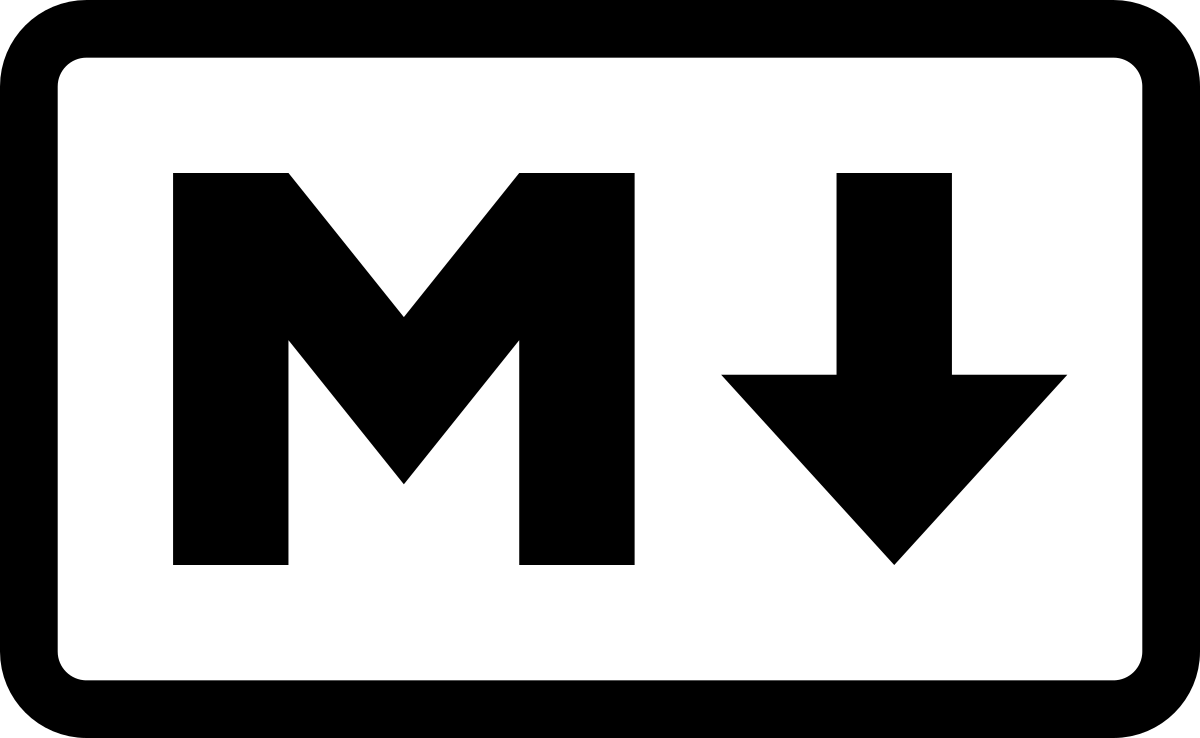
\includegraphics[scale=0.1]{mainmatter/images/research methodology/markdown.png}
    \caption{Markdown logo}
    \label{fig:markdown}
\end{figure}

\newpage
The system features 4 pages, which includes:

\begin{itemize}
    \item Home\\
    The landing page showcases a brief introduction of the system, and the purpose of the system.\\
    \item About Project\\
    This page details of the project, where it presents the overview of the project, its dataset, and the model.\\
    \item Findings\\
    This page presents the findings of the project, where it showcases the accuracy and loss of the model, as well as the confusion matrix of the project.\\
    \item Demo\\
    This page allows users to test the system out, by uploading an image of a handwriting sample, and the system will predict the class of the handwriting sample.\\
\end{itemize}

The system is presented in a custom dark-coloured theme, with lime green as the accent colour. The system is made responsive, where it can be viewed on mobile devices, as well as desktops. The system is hosted on Streamlit Community Cloud.

% The structure of the system can be seen in Figure. The system is made up of 3 main components, which are the frontend, backend, and the model. The frontend is made using HTML, CSS, and JavaScript, while the backend is made using Express.js. The model is made using TensorFlow.js, which is loaded into the backend.

% With that, Express.js, a web application framework for Node.js, to present the results of the model. Express.js is a minimal and flexible Node.js web application framework that provides a robust set of features for web and mobile applications. It is a lightweight framework that allows for the creation of single-page, multi-page, and hybrid web applications.

% \begin{figure}[h]
%     \centering
%     
\includegraphics[scale=0.4]{mainmatter/images/research methodology/expressjs.png}
%     \caption{Express.js logo}
%     \label{fig:expressjs}
% \end{figure}

% To allow the usage of the trained model, TensorFlow.js was used, specifically, a version that is made for Node.js that utilises GPU acceleration. The model was converted to a format that is compatible with TensorFlow.js, which is a \texttt{.json} file. This allows for the model to be loaded into the system, and be used to predict the class of the input image.

% In the early stages of developing the system, to ensure that the model is working as intended, the system only consists of the model and the backend. The model was loaded into the backend, and the backend was used to predict the class of the input image, through a simple interface. The input image was sent to the backend via a POST request, and the backend will return the predicted class of the input image, in the form of a JSON object. 

% \begin{figure}[h]
%     \centering
%     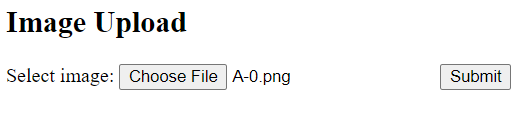
\includegraphics[scale=0.7]{mainmatter/images/research methodology/form.png}
%     \caption{Initial upload form}
%     \label{fig:uploadform}
% \end{figure}

% \begin{figure}[h]
%     \centering
%     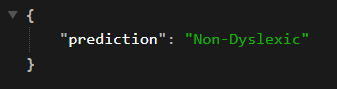
\includegraphics[scale=0.7]{mainmatter/images/research methodology/json_result.png}
%     \caption{JSON output}
%     \label{fig:jsonoutput}
% \end{figure}

% The overall navigation structure of the system is kept simple, with the main page being the homepage, which contains a brief introduction of the system. The other page is the prediction page, where the user can upload an image to be predicted. 


\newpage
\section{Documentation}
The final phase of the study is the documentation phase, where all completed tasks were recorded. This involves the preparation of a comprehensive final report detailing each and every activities carried out during this research. The final report represents an culmination of all information and discoveries related to the project's implementation and development, serving as a complete record of the project's execution.

\begin{figure}[h]
    \centering
    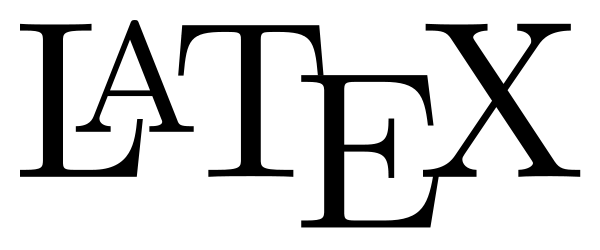
\includegraphics[scale=0.3]{mainmatter/images/research methodology/LaTeX_logo.png}
    \caption{LaTeX logo}
    \label{fig:latex}
\end{figure}

The documentation is made possible via \LaTeX, a document preparation system for high-quality typesetting. It is most often used for medium-to-large technical or scientific documents but it can be used for almost any form of publishing. \LaTeX is not a word processor, but rather a document markup language. For this project, a template made by \textcite{Rizauddin2023} was used as a base for the documentation, with a few changes made to adapt to the Final Year Project format. 

\newpage
\section{Summary}
In conclusion, this chapter goes through the research methodologies that has been applied throughout the research. This chapter details all the phases that will be involved from the start to finish. It also provides an mental image of how the flow of the study went.

% A Gantt chart visualizing the flow of the entire study was made, based on the phases of the research, as shown in the figure below:

% \newpage
% \thispagestyle{empty}
% \begin{landscape}

% \begin{figure}[h]
%     \begin{center}
    
%     \begin{ganttchart}[y unit title=0.7cm,
%     y unit chart=0.5cm,
%     vgrid,hgrid, 
%     title label anchor/.style={below=-1.6ex},
%     title left shift=.05,
%     title right shift=-.05,
%     title height=1,
%     progress label text={},
%     bar height=0.7,
%     group right shift=0,
%     group top shift=.6,
%     group height=.3]{1}{28}
%     %labels
%     \gantttitle{Semester 5}{14}
%     \gantttitle{Semester 6}{14}\\
%     \gantttitle{1}{1} 
%     \gantttitle{2}{1} 
%     \gantttitle{3}{1} 
%     \gantttitle{4}{1} 
%     \gantttitle{5}{1} 
%     \gantttitle{6}{1} 
%     \gantttitle{7}{1}
%     \gantttitle{8}{1}
%     \gantttitle{9}{1}
%     \gantttitle{10}{1}
%     \gantttitle{11}{1}
%     \gantttitle{12}{1}
%     \gantttitle{13}{1}
%     \gantttitle{14}{1}
%     \gantttitle{1}{1} 
%     \gantttitle{2}{1} 
%     \gantttitle{3}{1} 
%     \gantttitle{4}{1} 
%     \gantttitle{5}{1} 
%     \gantttitle{6}{1} 
%     \gantttitle{7}{1}
%     \gantttitle{8}{1}
%     \gantttitle{9}{1}
%     \gantttitle{10}{1}
%     \gantttitle{11}{1}
%     \gantttitle{12}{1}
%     \gantttitle{13}{1}
%     \gantttitle{14}{1}
%     \\
%     %tasks
%     \ganttbar{Preliminary Study}{1}{5} \\
%     \ganttbar{Knowledge Acquisition}{6}{14} \\
%     \ganttbar{Data Collection}{15}{15} \\
%     \ganttbar{Data Pre-processing}{16}{17} \\
%     \ganttbar{Model Development}{18}{22} \\
%     \ganttbar{Model Testing and Evaluation}{23}{25} \\
%     \ganttbar{System Development}{26}{28}\\
%     \ganttbar{Documentation}{1}{28}
    
%     % %relations 
%     % \ganttlink{elem0}{elem1} 
%     % \ganttlink{elem0}{elem3} 
%     % \ganttlink{elem1}{elem2} 
%     % \ganttlink{elem3}{elem4} 
%     % \ganttlink{elem1}{elem5} 
%     % \ganttlink{elem3}{elem5} 
%     % \ganttlink{elem2}{elem6} 
%     % \ganttlink{elem3}{elem6} 
%     \end{ganttchart}
%     \end{center}
%     \caption{Gantt Chart}
%     \label{ganttchart}

% \end{figure}
% \end{landscape}


% \section{Study Area}

% \section{Sampling}


% \begin{table}[ht]
%     \caption{My Sample}
%     \begin{tabular}{cc}
%         \toprule %header
%         \textbf{Millimeters} & \textbf{Centimeters}\\
%         \textbf{mm}          &   \textbf{cm}\\
%         \midrule
%         1           &   0.1\\ \hline
%         10          &   1\\ \hline
%         100         &   10\\ \hline
%         1000        &   100\\ \hline
%         10000       &   1000\\
%         \bottomrule
%     \end{tabular}
%     \par\raggedright Note: This table is useful for $\ldots$.
%     \label{tab:my_label}
% \end{table}

% \begin{table}[ht]
%     \caption{The Second Sample}
%     \begin{tabular}{>{\centering\arraybackslash}p{.47\textwidth} >{\centering\arraybackslash}p{.47\textwidth}}
%         \toprule %header
%         \textbf{Millimeters} & \textbf{Centimeters}\\
%         \textbf{mm}          &   \textbf{cm}\\
%         \midrule
%         1           &   0.1\\ \hline
%         10          &   1\\ \hline
%         100         &   10\\ \hline
%         1000        &   100\\ \hline
%         10000       &   1000\\
%         \bottomrule
%     \end{tabular}
%     \par\raggedright Note: This table is useful for $\ldots$.
%     \label{tab:my_second_label}
% \end{table}

% \begin{figure}[ht]
%     \centering
%     \fbox{%
%         
\includegraphics{mainmatter/images/logouitm.png}
%     }
%     \caption{A New Figure Again!}
%     \label{fig:newfig}
% \end{figure}

% \lipsum[2]

% \begin{figure}[ht]
%     \centering
%     \begin{tabular}{|c|c|}
%     \hline
%      \begin{subfigure}[b]{0.44\textwidth}
%          \centering
%          
\includegraphics[width=.8\linewidth]{mainmatter/images/logouitm.png}
%          \caption{$y=x$}
%          \label{fig:y_equals_x}
%      \end{subfigure} &
%      \begin{subfigure}[b]{0.44\textwidth}
%          \centering
%          
\includegraphics[width=.8\linewidth]{mainmatter/images/logouitm.png}
%          \caption{$x=y$}
%          \label{fig:x_equals_y}
%      \end{subfigure} \\
%      \hline
%     \end{tabular}
%     \caption{The Two Figures}
%     \label{fig:the2fig}
% \end{figure}

% \lipsum[1]

% \begin{figure}[ht]
%     \centering
% 	\begin{tabular}{|c|c|}
% 		\hline
% 		\begin{subfigure}[b]{0.44\textwidth}
% 			\centering
% 			
\includegraphics[width=.8\linewidth]{mainmatter/images/logouitm.png}
% 			\caption{$x=y$}
%          	\label{fig:x_equals_y4}
% 		\end{subfigure} & 
% 				\begin{subfigure}[b]{0.44\textwidth}
% 			\centering
% 			
\includegraphics[width=.8\linewidth]{mainmatter/images/logouitm.png}
% 			\caption{$x=y$}
%          	\label{fig:xy_equals_y3}
% 		\end{subfigure}	\\
% 		\hline
% 		\begin{subfigure}[b]{0.44\textwidth}
% 			\centering
% 			
\includegraphics[width=.8\linewidth]{mainmatter/images/logouitm.png}
% 			\caption{$x=y$}
%          	\label{fig:yy1}
% 		\end{subfigure} & 
% 				\begin{subfigure}[b]{0.44\textwidth}
% 			\centering
% 			
\includegraphics[width=.8\linewidth]{mainmatter/images/logouitm.png}
% 			\caption{$x=y$}
%          	\label{fig:xy2}
% 		\end{subfigure}	\\
% 		\hline		
% 	\end{tabular}
%     \caption{The Four Figures}
%     \label{fig:the4fig}
% \end{figure}


% \begin{landscape}

% \begin{figure}[ht]
%     \centering
% 	\begin{tabular}{|c|c|c|}
% 		\hline
% 		\begin{subfigure}[b]{0.44\textwidth}
% 			\centering
% 			\includegraphics[width=.8\linewidth]{example-image-a.jpg}
% 			\caption{$x=y$}
%          	\label{fig:ly1}
% 		\end{subfigure} & 
% 		\begin{subfigure}[b]{0.44\textwidth}
% 			\centering
% 			\includegraphics[width=.8\linewidth]{example-image-b.jpg}
% 			\caption{$x=y$}
%          	\label{fig:ly2}
% 		\end{subfigure} & 
% 		\begin{subfigure}[b]{0.44\textwidth}
% 			\centering
% 			\includegraphics[width=.8\linewidth]{example-image-c.jpg}
% 			\caption{$x=y$}
%          	\label{fig:ly3}
% 		\end{subfigure}\\
% 		\hline
% 		\begin{subfigure}[b]{0.44\textwidth}
% 			\centering
% 			
\includegraphics[width=.8\linewidth]{mainmatter/images/logouitm.png}
% 			\caption{$x=y$}
%          	\label{fig:ly4}
% 		\end{subfigure} & 
% 		\begin{subfigure}[b]{0.44\textwidth}
% 			\centering
% 			
\includegraphics[width=.8\linewidth]{mainmatter/images/logouitm.png}
% 			\caption{$x=y$}
%          	\label{fig:ly5}
% 		\end{subfigure} & 
% 		\begin{subfigure}[b]{0.44\textwidth}
% 			\centering
% 			
\includegraphics[width=.8\linewidth]{mainmatter/images/logouitm.png}
% 			\caption{$x=y$}
%          	\label{fig:ly6}
% 		\end{subfigure}\\
% 		\hline
% 		\begin{subfigure}[b]{0.44\textwidth}
% 			\centering
% 			\includegraphics[width=.8\linewidth]{example-image-a.jpg}
% 			\caption{$x=y$}
%          	\label{fig:ly7}
% 		\end{subfigure} & 
% 		\begin{subfigure}[b]{0.44\textwidth}
% 			\centering
% 			\includegraphics[width=.8\linewidth]{example-image-b.jpg}
% 			\caption{$x=y$}
%          	\label{fig:ly8}
% 		\end{subfigure} & 
% 		\begin{subfigure}[b]{0.44\textwidth}
% 			\centering
% 			\includegraphics[width=.8\linewidth]{example-image-c.jpg}
% 			\caption{$x=y$}
%          	\label{fig:ly9}
% 		\end{subfigure}\\
% 		\hline
% 	\end{tabular}	      
%     \caption{The Landscape Figures}
%     \label{fig:my_label_landscape}
% \end{figure}

% \end{landscape}

% \lipsum[1]